\documentclass[12pt]{exam}
%\documentclass[12pt]{article}
\usepackage[letterpaper, margin=0.75in]{geometry}
\usepackage{graphicx}
\usepackage{enumitem}
\usepackage{booktabs}
\usepackage{amsmath}
\usepackage{tabularx}
\usepackage{color}
\usepackage{textcomp}

\begin{document}
\footer{}{Page \thepage\ of \numpages}{}

\begin{flushright}
\makebox[0.5\textwidth]{\large Name:\enspace\hrulefill}
\vspace{0.2in}

\makebox[0.5\textwidth]{\large Date:\enspace\hrulefill}
\end{flushright}

\begin{center}

\includegraphics[width=10cm]{../images/logo.png}
\end{center}

\begin{center}
\noindent{\LARGE Conceptual Physics \\ Class 5 Questions \\ March 2, 2018 \\}
\end{center}
\vspace{0.2in}

Below is a cartoon picture of the atom, following the atomic model that makes it look like planets:

\noindent \begin{center}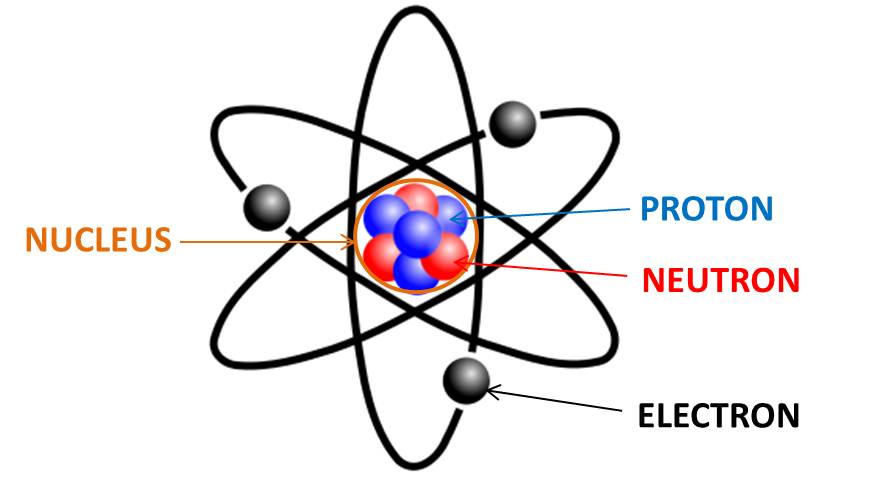
\includegraphics[width=4in]{../images/atom.jpg}\end{center}

Where the \textit{nucleus} is located in the middle of the atom and is orbited by electrons. Protons are \textit{POSIT}ively charged, neutrons carry no charge (\textit{NEUT}ral) and electron are negatively charged (and named for archaic reasons having to due with Greeks and tree resin). Electrons are \textit{fundamental particles} - they cannot (to our knowledge) be further broken down. Protons and neutron, however, are composite particles, meaning that they can be further broken down. \textit{Quarks} come together to form protons and neutrons, and are themselves fundamental particles (discussed in Chapter 0 of \textit{Light and Matter} and chapter 33, section 5 of \textit{College Physics}).


\clearpage
\begin{center}
\begin{figure}
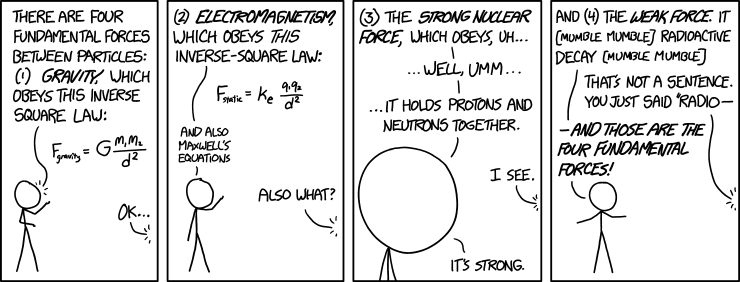
\includegraphics[width=\textwidth]{../images/xkcd_fundamental_forces.png}
\caption{``Of these four forces, there's one we don't really understand.'' ``Is it the weak force or the strong--'' ``It's gravity.'' (\textcopyright ~xkcd)}
\end{figure}
\end{center}
\begin{questions}
\question
	\begin{parts}
		\part How does the gravitational force vary with mass and distance?
			\vspace{1in}
		\part How does the electric force vary with electric charge and distance?
			\vspace{1in}
		\part Why do we not notice the nuclear forces in our everyday lives?
			\vspace{1in}
	\end{parts}
	
\clearpage
\question Nuclei come with a variety of different numbers of protons, ranging from 1 to about 110. The number of neutrons extends over a wider range, 0 to more than 150. However, nuclei which consist only of protons do not exist, except for hydrogen (which has 1 proton). Very massive nuclei exist only in forms for which the neutrons outnumber the protons.
\begin{parts}
\part What are the forces acting between two protons? Between a proton and a neutron? Between two neutrons?
\vspace{1in}
\part How does the net force between a proton and a neutron differ from that between two protons?
\vspace{1in}
\part Could an ``all-proton'' nucleus ever result in a net force that is repulsive for the protons? How might that occur?
\vspace{1in}
\part Use the answers from (a)-(c) to explain why neutrons must be present in the nucleus. Feel free to draw diagrams.
\end{parts}
\vspace{1in}

\clearpage
\question Two identical planets, planet A and planet B, are orbiting a star. Planet A is located twice as far away from the star as planet B.
	\begin{parts}
	\part Which one experiences the greater gravitational force from the star?
	\begin{center}\input{../images/solarSystem.pdf_tex}\end{center}
	\part How much greater is this force?
	\end{parts}

\clearpage
\question Gravity can be used to explain the ocean tides, by considering the gravitational pull of the moon.
\begin{center}
\input{../images/tides.pdf_tex}
\end{center}
\begin{parts}
	\part In the above diagram, which part of the earth (A, B, C, D) experiences the greatest force from the moon?
		\vspace{0.25in}
	\part What impact does this have on the ocean?
		\vspace{1in}
	\part As the moon orbits around the earth, what happens? Note: Something important happens on the side \textit{opposite} to that of the moon.
		\vspace{1in}
	\part What causes the ocean tides?
		\vspace{1in}
\end{parts}

\clearpage
\question When you hold up a rock, and drop it, you notice the rock accelerates down.
\begin{parts}
	\part What is the main force acting on the rock?
		\vspace{1in}
	\part What is the other object interacting with the rock?
		\vspace{1in}
	\part Newton's third law states that for every action, there is an equal and opposite reaction. What does that mean in this scenario?
		\vspace{1in}
	\part Why don't we notice this ``reaction" pair?
		\vspace{1in}
		
\end{parts}
\question A 60~kg sprinter starts a race with an acceleration of $4~m/s^2$.
	\begin{parts}	
	\part What is the net force on the sprinter?
		\vspace{1in}
	\part If the sprinter maintains this acceleration for 18~m, what is their final velocity?
		\vspace{1in}
	\end{parts}

\clearpage

\question
Oscilloscopes and old-fashioned televisions use a series of electrical forces to create a picture. Electrons hit a screen and create light. The color of the light depends on the type of atom struck by the electron. Electrical forces are used to get the electron the place it is needed. The diagram below illustrates just such a setup:

\begin{center}
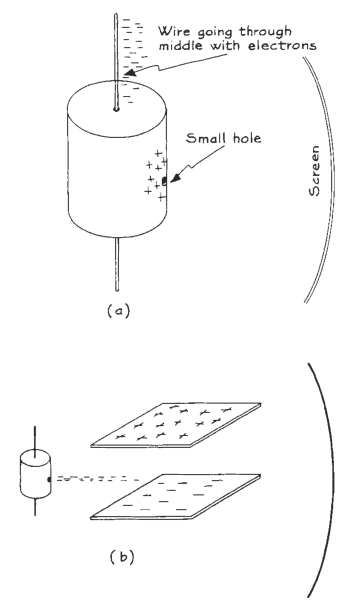
\includegraphics[width=2in]{../images/oscilloscopes.png}
\end{center}

\begin{parts}
	\part The first step is to get electrons moving. The basic setup is shown in (a). Why does this arrangement result in a bright spot on the screen as shown? (This arrangement is called an electron gun).
	\vspace{1in}
	
	\part Looking at bright spots on screens is not very exciting, so we must move the electrons. How does the arrangement in (b) change the motion of the electrons?
	\vspace{1in}
	
	\part In television the charge on the deflecting plates changes from positive on the top and negative on the bottom to positive on the bottom and negative on the top in 1/60~s. The change is gradual, not sudden. What will be the motion of the electrons?
	\vspace{1in}
\end{parts}

\end{questions}

\end{document}


\end{document}
